\documentclass[twoside]{book}

% Packages required by doxygen
\usepackage{fixltx2e}
\usepackage{calc}
\usepackage{doxygen}
\usepackage[export]{adjustbox} % also loads graphicx
\usepackage{graphicx}
\usepackage[utf8]{inputenc}
\usepackage{makeidx}
\usepackage{multicol}
\usepackage{multirow}
\PassOptionsToPackage{warn}{textcomp}
\usepackage{textcomp}
\usepackage[nointegrals]{wasysym}
\usepackage[table]{xcolor}

% Font selection
\usepackage[T1]{fontenc}
\usepackage[scaled=.90]{helvet}
\usepackage{courier}
\usepackage{amssymb}
\usepackage{sectsty}
\renewcommand{\familydefault}{\sfdefault}
\allsectionsfont{%
  \fontseries{bc}\selectfont%
  \color{darkgray}%
}
\renewcommand{\DoxyLabelFont}{%
  \fontseries{bc}\selectfont%
  \color{darkgray}%
}
\newcommand{\+}{\discretionary{\mbox{\scriptsize$\hookleftarrow$}}{}{}}

% Page & text layout
\usepackage{geometry}
\geometry{%
  a4paper,%
  top=2.5cm,%
  bottom=2.5cm,%
  left=2.5cm,%
  right=2.5cm%
}
\tolerance=750
\hfuzz=15pt
\hbadness=750
\setlength{\emergencystretch}{15pt}
\setlength{\parindent}{0cm}
\setlength{\parskip}{3ex plus 2ex minus 2ex}
\makeatletter
\renewcommand{\paragraph}{%
  \@startsection{paragraph}{4}{0ex}{-1.0ex}{1.0ex}{%
    \normalfont\normalsize\bfseries\SS@parafont%
  }%
}
\renewcommand{\subparagraph}{%
  \@startsection{subparagraph}{5}{0ex}{-1.0ex}{1.0ex}{%
    \normalfont\normalsize\bfseries\SS@subparafont%
  }%
}
\makeatother

% Headers & footers
\usepackage{fancyhdr}
\pagestyle{fancyplain}
\fancyhead[LE]{\fancyplain{}{\bfseries\thepage}}
\fancyhead[CE]{\fancyplain{}{}}
\fancyhead[RE]{\fancyplain{}{\bfseries\leftmark}}
\fancyhead[LO]{\fancyplain{}{\bfseries\rightmark}}
\fancyhead[CO]{\fancyplain{}{}}
\fancyhead[RO]{\fancyplain{}{\bfseries\thepage}}
\fancyfoot[LE]{\fancyplain{}{}}
\fancyfoot[CE]{\fancyplain{}{}}
\fancyfoot[RE]{\fancyplain{}{\bfseries\scriptsize Generated by Doxygen }}
\fancyfoot[LO]{\fancyplain{}{\bfseries\scriptsize Generated by Doxygen }}
\fancyfoot[CO]{\fancyplain{}{}}
\fancyfoot[RO]{\fancyplain{}{}}
\renewcommand{\footrulewidth}{0.4pt}
\renewcommand{\chaptermark}[1]{%
  \markboth{#1}{}%
}
\renewcommand{\sectionmark}[1]{%
  \markright{\thesection\ #1}%
}

% Indices & bibliography
\usepackage{natbib}
\usepackage[titles]{tocloft}
\setcounter{tocdepth}{3}
\setcounter{secnumdepth}{5}
\makeindex

% Hyperlinks (required, but should be loaded last)
\usepackage{ifpdf}
\ifpdf
  \usepackage[pdftex,pagebackref=true]{hyperref}
\else
  \usepackage[ps2pdf,pagebackref=true]{hyperref}
\fi
\hypersetup{%
  colorlinks=true,%
  linkcolor=blue,%
  citecolor=blue,%
  unicode%
}

% Custom commands
\newcommand{\clearemptydoublepage}{%
  \newpage{\pagestyle{empty}\cleardoublepage}%
}

\usepackage{caption}
\captionsetup{labelsep=space,justification=centering,font={bf},singlelinecheck=off,skip=4pt,position=top}

%===== C O N T E N T S =====

\begin{document}

% Titlepage & ToC
\hypersetup{pageanchor=false,
             bookmarksnumbered=true,
             pdfencoding=unicode
            }
\pagenumbering{alph}
\begin{titlepage}
\vspace*{7cm}
\begin{center}%
{\Large Leet\+Translator }\\
\vspace*{1cm}
{\large Generated by Doxygen 1.8.14}\\
\end{center}
\end{titlepage}
\clearemptydoublepage
\pagenumbering{roman}
\tableofcontents
\clearemptydoublepage
\pagenumbering{arabic}
\hypersetup{pageanchor=true}

%--- Begin generated contents ---
\chapter{Namespace Index}
\section{Packages}
Here are the packages with brief descriptions (if available)\+:\begin{DoxyCompactList}
\item\contentsline{section}{\mbox{\hyperlink{namespace_leet_translator_grafica}{Leet\+Translator\+Grafica}} }{\pageref{namespace_leet_translator_grafica}}{}
\end{DoxyCompactList}

\chapter{Hierarchical Index}
\section{Class Hierarchy}
This inheritance list is sorted roughly, but not completely, alphabetically\+:\begin{DoxyCompactList}
\item Application\begin{DoxyCompactList}
\item \contentsline{section}{Leet\+Translator\+Grafica.\+App}{\pageref{class_leet_translator_grafica_1_1_app}}{}
\end{DoxyCompactList}
\item \contentsline{section}{Leet\+Translator\+Grafica.\+Translator}{\pageref{class_leet_translator_grafica_1_1_translator}}{}
\item Window\begin{DoxyCompactList}
\item \contentsline{section}{Leet\+Translator\+Grafica.\+Main\+Window}{\pageref{class_leet_translator_grafica_1_1_main_window}}{}
\end{DoxyCompactList}
\end{DoxyCompactList}

\chapter{Class Index}
\section{Class List}
Here are the classes, structs, unions and interfaces with brief descriptions\+:\begin{DoxyCompactList}
\item\contentsline{section}{\mbox{\hyperlink{class_leet_translator_grafica_1_1_app}{Leet\+Translator\+Grafica.\+App}} \\*Logica di interazione per App.\+xaml }{\pageref{class_leet_translator_grafica_1_1_app}}{}
\item\contentsline{section}{\mbox{\hyperlink{class_leet_translator_grafica_1_1_main_window}{Leet\+Translator\+Grafica.\+Main\+Window}} \\*Logica di interazione per Main\+Window.\+xaml }{\pageref{class_leet_translator_grafica_1_1_main_window}}{}
\item\contentsline{section}{\mbox{\hyperlink{class_leet_translator_grafica_1_1_translator}{Leet\+Translator\+Grafica.\+Translator}} \\*Class that represents a translator and perform translations }{\pageref{class_leet_translator_grafica_1_1_translator}}{}
\end{DoxyCompactList}

\chapter{Namespace Documentation}
\hypertarget{namespace_leet_translator_grafica}{}\section{Leet\+Translator\+Grafica Namespace Reference}
\label{namespace_leet_translator_grafica}\index{Leet\+Translator\+Grafica@{Leet\+Translator\+Grafica}}
\subsection*{Classes}
\begin{DoxyCompactItemize}
\item 
class \mbox{\hyperlink{class_leet_translator_grafica_1_1_app}{App}}
\begin{DoxyCompactList}\small\item\em Logica di interazione per App.\+xaml \end{DoxyCompactList}\item 
class \mbox{\hyperlink{class_leet_translator_grafica_1_1_main_window}{Main\+Window}}
\begin{DoxyCompactList}\small\item\em Logica di interazione per Main\+Window.\+xaml \end{DoxyCompactList}\item 
class \mbox{\hyperlink{class_leet_translator_grafica_1_1_translator}{Translator}}
\begin{DoxyCompactList}\small\item\em Class that represents a translator and perform translations \end{DoxyCompactList}\end{DoxyCompactItemize}

\chapter{Class Documentation}
\hypertarget{class_leet_translator_grafica_1_1_app}{}\section{Leet\+Translator\+Grafica.\+App Class Reference}
\label{class_leet_translator_grafica_1_1_app}\index{Leet\+Translator\+Grafica.\+App@{Leet\+Translator\+Grafica.\+App}}


Logica di interazione per App.\+xaml  


Inheritance diagram for Leet\+Translator\+Grafica.\+App\+:\begin{figure}[H]
\begin{center}
\leavevmode
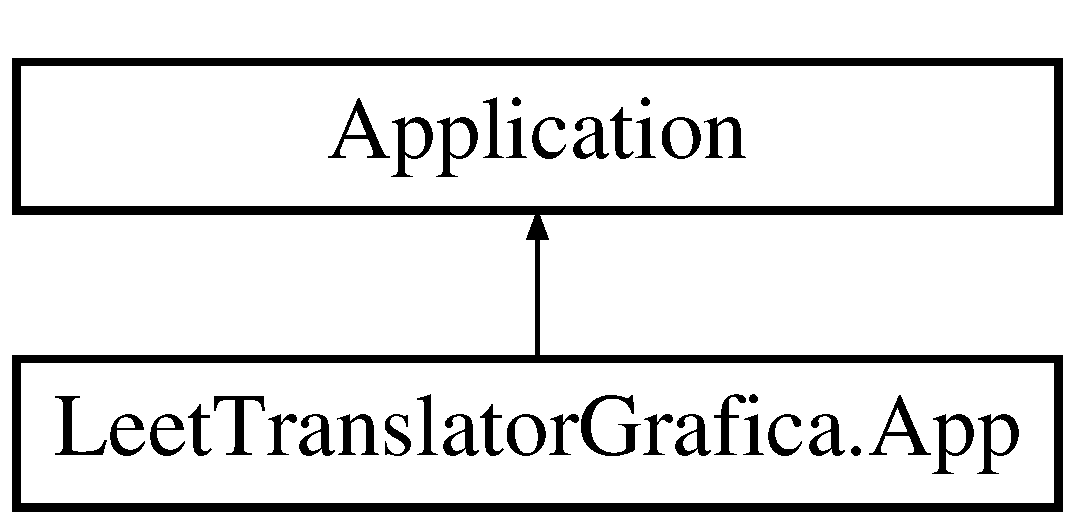
\includegraphics[height=2.000000cm]{class_leet_translator_grafica_1_1_app}
\end{center}
\end{figure}


\subsection{Detailed Description}
Logica di interazione per App.\+xaml 



The documentation for this class was generated from the following file\+:\begin{DoxyCompactItemize}
\item 
D\+:/alex2/\+Desktop/\+Leet\+Translator/\+G\+U\+I Project/\+Leet\+Translator\+Grafica/App.\+xaml.\+cs\end{DoxyCompactItemize}

\hypertarget{class_leet_translator_grafica_1_1_main_window}{}\section{Leet\+Translator\+Grafica.\+Main\+Window Class Reference}
\label{class_leet_translator_grafica_1_1_main_window}\index{Leet\+Translator\+Grafica.\+Main\+Window@{Leet\+Translator\+Grafica.\+Main\+Window}}


Logica di interazione per Main\+Window.\+xaml  


Inheritance diagram for Leet\+Translator\+Grafica.\+Main\+Window\+:\begin{figure}[H]
\begin{center}
\leavevmode
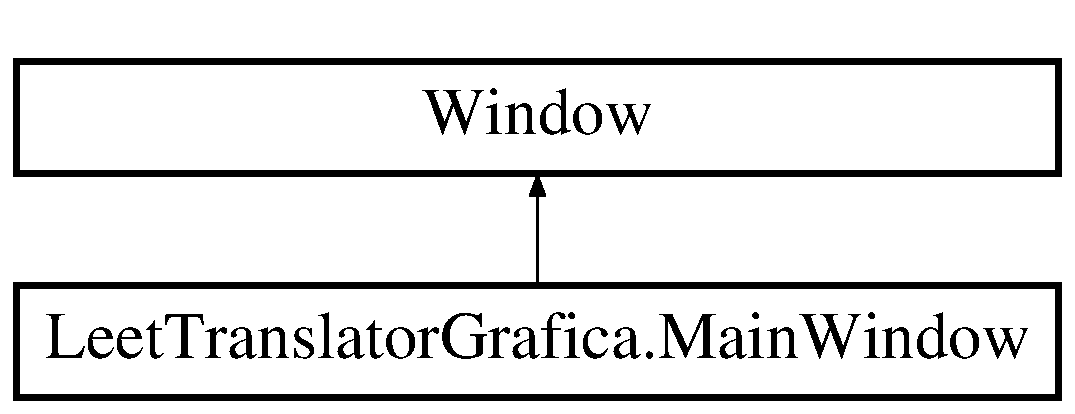
\includegraphics[height=2.000000cm]{class_leet_translator_grafica_1_1_main_window}
\end{center}
\end{figure}
\subsection*{Private Member Functions}
\begin{DoxyCompactItemize}
\item 
void \mbox{\hyperlink{class_leet_translator_grafica_1_1_main_window_a421197948c143ef1794985b934dff9b1}{translate\+Btn\+\_\+\+Click}} (object sender, Routed\+Event\+Args e)
\begin{DoxyCompactList}\small\item\em Start the translation process \end{DoxyCompactList}\item 
void \mbox{\hyperlink{class_leet_translator_grafica_1_1_main_window_aceeed66386ce7e420d4664e9d216f77c}{window\+\_\+\+Loaded\+\_\+1}} (object sender, Routed\+Event\+Args e)
\begin{DoxyCompactList}\small\item\em Perform when the window is loaded \end{DoxyCompactList}\item 
void \mbox{\hyperlink{class_leet_translator_grafica_1_1_main_window_a42997ac15b81e590c852a728d2959ee9}{clear\+Btn\+\_\+\+Click}} (object sender, Routed\+Event\+Args e)
\begin{DoxyCompactList}\small\item\em Clean text field \end{DoxyCompactList}\item 
void \mbox{\hyperlink{class_leet_translator_grafica_1_1_main_window_a4a643cadb0b1b10c0e7489d007c088a2}{info\+Btn\+\_\+\+Click}} (object sender, Routed\+Event\+Args e)
\begin{DoxyCompactList}\small\item\em Show info about this software \end{DoxyCompactList}\end{DoxyCompactItemize}


\subsection{Detailed Description}
Logica di interazione per Main\+Window.\+xaml 



\subsection{Member Function Documentation}
\mbox{\Hypertarget{class_leet_translator_grafica_1_1_main_window_a42997ac15b81e590c852a728d2959ee9}\label{class_leet_translator_grafica_1_1_main_window_a42997ac15b81e590c852a728d2959ee9}} 
\index{Leet\+Translator\+Grafica\+::\+Main\+Window@{Leet\+Translator\+Grafica\+::\+Main\+Window}!clear\+Btn\+\_\+\+Click@{clear\+Btn\+\_\+\+Click}}
\index{clear\+Btn\+\_\+\+Click@{clear\+Btn\+\_\+\+Click}!Leet\+Translator\+Grafica\+::\+Main\+Window@{Leet\+Translator\+Grafica\+::\+Main\+Window}}
\subsubsection{\texorpdfstring{clear\+Btn\+\_\+\+Click()}{clearBtn\_Click()}}
{\footnotesize\ttfamily void Leet\+Translator\+Grafica.\+Main\+Window.\+clear\+Btn\+\_\+\+Click (\begin{DoxyParamCaption}\item[{object}]{sender,  }\item[{Routed\+Event\+Args}]{e }\end{DoxyParamCaption})\hspace{0.3cm}{\ttfamily [private]}}



Clean text field 


\begin{DoxyParams}{Parameters}
{\em sender} & \\
\hline
{\em e} & \\
\hline
\end{DoxyParams}
\mbox{\Hypertarget{class_leet_translator_grafica_1_1_main_window_a4a643cadb0b1b10c0e7489d007c088a2}\label{class_leet_translator_grafica_1_1_main_window_a4a643cadb0b1b10c0e7489d007c088a2}} 
\index{Leet\+Translator\+Grafica\+::\+Main\+Window@{Leet\+Translator\+Grafica\+::\+Main\+Window}!info\+Btn\+\_\+\+Click@{info\+Btn\+\_\+\+Click}}
\index{info\+Btn\+\_\+\+Click@{info\+Btn\+\_\+\+Click}!Leet\+Translator\+Grafica\+::\+Main\+Window@{Leet\+Translator\+Grafica\+::\+Main\+Window}}
\subsubsection{\texorpdfstring{info\+Btn\+\_\+\+Click()}{infoBtn\_Click()}}
{\footnotesize\ttfamily void Leet\+Translator\+Grafica.\+Main\+Window.\+info\+Btn\+\_\+\+Click (\begin{DoxyParamCaption}\item[{object}]{sender,  }\item[{Routed\+Event\+Args}]{e }\end{DoxyParamCaption})\hspace{0.3cm}{\ttfamily [private]}}



Show info about this software 


\begin{DoxyParams}{Parameters}
{\em sender} & \\
\hline
{\em e} & \\
\hline
\end{DoxyParams}
\mbox{\Hypertarget{class_leet_translator_grafica_1_1_main_window_a421197948c143ef1794985b934dff9b1}\label{class_leet_translator_grafica_1_1_main_window_a421197948c143ef1794985b934dff9b1}} 
\index{Leet\+Translator\+Grafica\+::\+Main\+Window@{Leet\+Translator\+Grafica\+::\+Main\+Window}!translate\+Btn\+\_\+\+Click@{translate\+Btn\+\_\+\+Click}}
\index{translate\+Btn\+\_\+\+Click@{translate\+Btn\+\_\+\+Click}!Leet\+Translator\+Grafica\+::\+Main\+Window@{Leet\+Translator\+Grafica\+::\+Main\+Window}}
\subsubsection{\texorpdfstring{translate\+Btn\+\_\+\+Click()}{translateBtn\_Click()}}
{\footnotesize\ttfamily void Leet\+Translator\+Grafica.\+Main\+Window.\+translate\+Btn\+\_\+\+Click (\begin{DoxyParamCaption}\item[{object}]{sender,  }\item[{Routed\+Event\+Args}]{e }\end{DoxyParamCaption})\hspace{0.3cm}{\ttfamily [private]}}



Start the translation process 


\begin{DoxyParams}{Parameters}
{\em sender} & \\
\hline
{\em e} & \\
\hline
\end{DoxyParams}
\mbox{\Hypertarget{class_leet_translator_grafica_1_1_main_window_aceeed66386ce7e420d4664e9d216f77c}\label{class_leet_translator_grafica_1_1_main_window_aceeed66386ce7e420d4664e9d216f77c}} 
\index{Leet\+Translator\+Grafica\+::\+Main\+Window@{Leet\+Translator\+Grafica\+::\+Main\+Window}!window\+\_\+\+Loaded\+\_\+1@{window\+\_\+\+Loaded\+\_\+1}}
\index{window\+\_\+\+Loaded\+\_\+1@{window\+\_\+\+Loaded\+\_\+1}!Leet\+Translator\+Grafica\+::\+Main\+Window@{Leet\+Translator\+Grafica\+::\+Main\+Window}}
\subsubsection{\texorpdfstring{window\+\_\+\+Loaded\+\_\+1()}{window\_Loaded\_1()}}
{\footnotesize\ttfamily void Leet\+Translator\+Grafica.\+Main\+Window.\+window\+\_\+\+Loaded\+\_\+1 (\begin{DoxyParamCaption}\item[{object}]{sender,  }\item[{Routed\+Event\+Args}]{e }\end{DoxyParamCaption})\hspace{0.3cm}{\ttfamily [private]}}



Perform when the window is loaded 


\begin{DoxyParams}{Parameters}
{\em sender} & \\
\hline
{\em e} & \\
\hline
\end{DoxyParams}


The documentation for this class was generated from the following file\+:\begin{DoxyCompactItemize}
\item 
D\+:/alex2/\+Desktop/\+Leet\+Translator/\+G\+U\+I Project/\+Leet\+Translator\+Grafica/Main\+Window.\+xaml.\+cs\end{DoxyCompactItemize}

\hypertarget{class_leet_translator_grafica_1_1_translator}{}\section{Leet\+Translator\+Grafica.\+Translator Class Reference}
\label{class_leet_translator_grafica_1_1_translator}\index{Leet\+Translator\+Grafica.\+Translator@{Leet\+Translator\+Grafica.\+Translator}}


Class that represents a translator and perform translations  


\subsection*{Static Public Member Functions}
\begin{DoxyCompactItemize}
\item 
static string \mbox{\hyperlink{class_leet_translator_grafica_1_1_translator_a5f13acd40cb9def2c45b69f98bd8935d}{Light\+Leet}} (string text)
\begin{DoxyCompactList}\small\item\em This alphabet uses symbols that are admitted by Windows in files\textquotesingle{} name \end{DoxyCompactList}\item 
static string \mbox{\hyperlink{class_leet_translator_grafica_1_1_translator_a0538325327e6153ea9d9ed2abbcf04aa}{Complete\+Leet}} (string text)
\begin{DoxyCompactList}\small\item\em This alphabet can use every symbols \end{DoxyCompactList}\item 
static void \mbox{\hyperlink{class_leet_translator_grafica_1_1_translator_a703defc4c40ffed8c59117dbabea532c}{Translate\+On\+File}} (string plain\+\_\+text, Func$<$ string, string $>$ translator)
\begin{DoxyCompactList}\small\item\em Write on file the translation \end{DoxyCompactList}\end{DoxyCompactItemize}
\subsection*{Private Member Functions}
\begin{DoxyCompactItemize}
\item 
\mbox{\hyperlink{class_leet_translator_grafica_1_1_translator_aa672be9ffa2be49533832a54185a86c5}{Translator}} ()
\begin{DoxyCompactList}\small\item\em Private constructor. This is a static class \end{DoxyCompactList}\end{DoxyCompactItemize}
\subsection*{Static Private Member Functions}
\begin{DoxyCompactItemize}
\item 
static \mbox{\hyperlink{class_leet_translator_grafica_1_1_translator_a196b667bf978f78c18068a0cde72cd67}{Translator}} ()
\begin{DoxyCompactList}\small\item\em Static initialize of the alphabet It has got two alphabet\+: light and complete \end{DoxyCompactList}\end{DoxyCompactItemize}
\subsection*{Private Attributes}
\begin{DoxyCompactItemize}
\item 
\mbox{\Hypertarget{class_leet_translator_grafica_1_1_translator_ad2fd30cbcd0e38c521c1c030611b4326}\label{class_leet_translator_grafica_1_1_translator_ad2fd30cbcd0e38c521c1c030611b4326}} 
const int {\bfseries N\+\_\+\+C\+H\+AR} = 256
\end{DoxyCompactItemize}
\subsection*{Static Private Attributes}
\begin{DoxyCompactItemize}
\item 
\mbox{\Hypertarget{class_leet_translator_grafica_1_1_translator_aa42f319a27433723c126ceb7d2db1e7b}\label{class_leet_translator_grafica_1_1_translator_aa42f319a27433723c126ceb7d2db1e7b}} 
static string \mbox{[}$\,$\mbox{]} {\bfseries light\+\_\+leet\+\_\+alphabet}
\item 
\mbox{\Hypertarget{class_leet_translator_grafica_1_1_translator_afd1909e5598e89e3a68c7c7d918a5452}\label{class_leet_translator_grafica_1_1_translator_afd1909e5598e89e3a68c7c7d918a5452}} 
static string \mbox{[}$\,$\mbox{]} {\bfseries complete\+\_\+leet\+\_\+alphabet}
\end{DoxyCompactItemize}


\subsection{Detailed Description}
Class that represents a translator and perform translations 



\subsection{Constructor \& Destructor Documentation}
\mbox{\Hypertarget{class_leet_translator_grafica_1_1_translator_a196b667bf978f78c18068a0cde72cd67}\label{class_leet_translator_grafica_1_1_translator_a196b667bf978f78c18068a0cde72cd67}} 
\index{Leet\+Translator\+Grafica\+::\+Translator@{Leet\+Translator\+Grafica\+::\+Translator}!Translator@{Translator}}
\index{Translator@{Translator}!Leet\+Translator\+Grafica\+::\+Translator@{Leet\+Translator\+Grafica\+::\+Translator}}
\subsubsection{\texorpdfstring{Translator()}{Translator()}\hspace{0.1cm}{\footnotesize\ttfamily [1/2]}}
{\footnotesize\ttfamily static Leet\+Translator\+Grafica.\+Translator.\+Translator (\begin{DoxyParamCaption}{ }\end{DoxyParamCaption})\hspace{0.3cm}{\ttfamily [static]}, {\ttfamily [private]}}



Static initialize of the alphabet It has got two alphabet\+: light and complete 

\mbox{\Hypertarget{class_leet_translator_grafica_1_1_translator_aa672be9ffa2be49533832a54185a86c5}\label{class_leet_translator_grafica_1_1_translator_aa672be9ffa2be49533832a54185a86c5}} 
\index{Leet\+Translator\+Grafica\+::\+Translator@{Leet\+Translator\+Grafica\+::\+Translator}!Translator@{Translator}}
\index{Translator@{Translator}!Leet\+Translator\+Grafica\+::\+Translator@{Leet\+Translator\+Grafica\+::\+Translator}}
\subsubsection{\texorpdfstring{Translator()}{Translator()}\hspace{0.1cm}{\footnotesize\ttfamily [2/2]}}
{\footnotesize\ttfamily Leet\+Translator\+Grafica.\+Translator.\+Translator (\begin{DoxyParamCaption}{ }\end{DoxyParamCaption})\hspace{0.3cm}{\ttfamily [private]}}



Private constructor. This is a static class 



\subsection{Member Function Documentation}
\mbox{\Hypertarget{class_leet_translator_grafica_1_1_translator_a0538325327e6153ea9d9ed2abbcf04aa}\label{class_leet_translator_grafica_1_1_translator_a0538325327e6153ea9d9ed2abbcf04aa}} 
\index{Leet\+Translator\+Grafica\+::\+Translator@{Leet\+Translator\+Grafica\+::\+Translator}!Complete\+Leet@{Complete\+Leet}}
\index{Complete\+Leet@{Complete\+Leet}!Leet\+Translator\+Grafica\+::\+Translator@{Leet\+Translator\+Grafica\+::\+Translator}}
\subsubsection{\texorpdfstring{Complete\+Leet()}{CompleteLeet()}}
{\footnotesize\ttfamily static string Leet\+Translator\+Grafica.\+Translator.\+Complete\+Leet (\begin{DoxyParamCaption}\item[{string}]{text }\end{DoxyParamCaption})\hspace{0.3cm}{\ttfamily [static]}}



This alphabet can use every symbols 


\begin{DoxyParams}{Parameters}
{\em text} & Text you want to translate\\
\hline
\end{DoxyParams}
\begin{DoxyReturn}{Returns}

\end{DoxyReturn}
\mbox{\Hypertarget{class_leet_translator_grafica_1_1_translator_a5f13acd40cb9def2c45b69f98bd8935d}\label{class_leet_translator_grafica_1_1_translator_a5f13acd40cb9def2c45b69f98bd8935d}} 
\index{Leet\+Translator\+Grafica\+::\+Translator@{Leet\+Translator\+Grafica\+::\+Translator}!Light\+Leet@{Light\+Leet}}
\index{Light\+Leet@{Light\+Leet}!Leet\+Translator\+Grafica\+::\+Translator@{Leet\+Translator\+Grafica\+::\+Translator}}
\subsubsection{\texorpdfstring{Light\+Leet()}{LightLeet()}}
{\footnotesize\ttfamily static string Leet\+Translator\+Grafica.\+Translator.\+Light\+Leet (\begin{DoxyParamCaption}\item[{string}]{text }\end{DoxyParamCaption})\hspace{0.3cm}{\ttfamily [static]}}



This alphabet uses symbols that are admitted by Windows in files\textquotesingle{} name 


\begin{DoxyParams}{Parameters}
{\em text} & Text you want to translate\\
\hline
\end{DoxyParams}
\begin{DoxyReturn}{Returns}

\end{DoxyReturn}
\mbox{\Hypertarget{class_leet_translator_grafica_1_1_translator_a703defc4c40ffed8c59117dbabea532c}\label{class_leet_translator_grafica_1_1_translator_a703defc4c40ffed8c59117dbabea532c}} 
\index{Leet\+Translator\+Grafica\+::\+Translator@{Leet\+Translator\+Grafica\+::\+Translator}!Translate\+On\+File@{Translate\+On\+File}}
\index{Translate\+On\+File@{Translate\+On\+File}!Leet\+Translator\+Grafica\+::\+Translator@{Leet\+Translator\+Grafica\+::\+Translator}}
\subsubsection{\texorpdfstring{Translate\+On\+File()}{TranslateOnFile()}}
{\footnotesize\ttfamily static void Leet\+Translator\+Grafica.\+Translator.\+Translate\+On\+File (\begin{DoxyParamCaption}\item[{string}]{plain\+\_\+text,  }\item[{Func$<$ string, string $>$}]{translator }\end{DoxyParamCaption})\hspace{0.3cm}{\ttfamily [static]}}



Write on file the translation 


\begin{DoxyParams}{Parameters}
{\em plain\+\_\+text} & Text you want to translate\\
\hline
{\em translator} & Function that allow you to translate\\
\hline
\end{DoxyParams}


The documentation for this class was generated from the following file\+:\begin{DoxyCompactItemize}
\item 
D\+:/alex2/\+Desktop/\+Leet\+Translator/\+G\+U\+I Project/\+Leet\+Translator\+Grafica/Translator.\+cs\end{DoxyCompactItemize}

%--- End generated contents ---

% Index
\backmatter
\newpage
\phantomsection
\clearemptydoublepage
\addcontentsline{toc}{chapter}{Index}
\printindex

\end{document}
